\documentclass[11pt]{article}

\usepackage{sbc-template}
\usepackage{graphicx,url}
\usepackage[utf8]{inputenc}
\usepackage[T1]{fontenc}
\usepackage{amsmath,amssymb}
\usepackage{listings}
\usepackage{float}
\usepackage{booktabs}
\usepackage{cite}

\renewcommand{\refname}{Referências}
\renewcommand{\figurename}{Figura}
\renewcommand{\tablename}{Tabela}

\lstset{
  basicstyle=\footnotesize\ttfamily,
  numbers=none,
  frame=lines,
  breaklines=true,
  keywordstyle=\bfseries\color{black},
  commentstyle=\itshape\color{black!70},
  tabsize=2,
  captionpos=t,
  escapeinside={(*@}{@*)}
}

\sloppy

\title{Meta-heurísticas Aplicadas ao Problema do Caixeiro Viajante:\\Estudo Comparativo com Têmpera Simulada e Algoritmos Genéticos}

\author{Mário Cordeiro Júnior\inst{1}, André F. Maccarini\inst{1}}

\address{Departamento Acadêmico de Informática (DAINF) \\
Universidade Tecnológica Federal do Paraná (UTFPR) -- Curitiba, PR -- Brasil
\email{mariojuniors31@gmail.com, andref.maccarini@gmail.com}
}

\begin{document} 

\maketitle

\begin{resumo} 
O Problema do Caixeiro Viajante (PCV) é um problema clássico de otimização combinatória NP-difícil com amplo espaço de busca. Este artigo investiga duas meta-heurísticas para a obtenção de soluções aproximadas em instâncias euclidianas simétricas: a Têmpera Simulada (TS), de trajetória única, e os Algoritmos Genéticos (AG), de base populacional. As decisões de projeto são descritas e justificadas em quatro níveis: domínio, modelagem, representação computacional e implementação. Avaliamos experimentalmente o comportamento dos algoritmos em instâncias de 20, 50 e 100 cidades, além de analisarmos 17 configurações com quatro funções de resfriamento na TS (linear, geométrico, exponencial e logarítmico). Os resultados demonstram a sensibilidade da TS à taxa de resfriamento, a eficácia do operador de cruzamento ordenado no AG para instâncias maiores e as vantagens de memória da busca local frente à explosão combinatorial do algoritmo $A^*$.
\end{resumo}

\begin{abstract}
The Traveling Salesperson Problem (TSP) is a classic NP-hard combinatorial optimization problem with a factorial state space. This paper evaluates two local search metaheuristics for approximate solutions on symmetric Euclidean instances: trajectory-based Simulated Annealing (SA) and population-based Genetic Algorithms (GA). Design choices are presented across four levels: domain, modeling, computational representation, and implementation. We evaluate both algorithms on 20, 50, and 100-city instances and examine 17 cooling configurations for SA covering linear, geometric, exponential, and logarithmic schedules. The results show the sensitivity of SA to temperature decay, the advantages of ordered crossover in GA on larger instances, and the memory scalability of local search over informed search ($A^*$).
\end{abstract}

\section{Introdução}

Na Inteligência Artificial, problemas de otimização podem ser formulados como busca em espaços de estados \cite{russell2022ia}. No Problema do Caixeiro Viajante (PCV), o objetivo é determinar um ciclo que visite um conjunto de cidades exatamente uma vez e retorne ao ponto de partida com custo total mínimo. Em instâncias simétricas com $n$ cidades, o número de rotas possíveis cresce fatorialmente, dado por $|S_n| = \frac{(n-1)!}{2}$ \cite{campello1994algoritmos}. Para $n=20$, existem mais de $6 \times 10^{16}$ rotas distintas; para $n=50$, esse número ultrapassa $3 \times 10^{62}$, inviabilizando a enumeração exaustiva.

Algoritmos exatos de busca informada, como o $A^*$, garantem a otimalidade global por meio de heurísticas admissíveis (como a Árvore Geradora Mínima). Contudo, a necessidade de armazenar caminhos parciais na fronteira de busca acarreta consumo exponencial de memória ($O(b^d)$). Na prática, o $A^*$ esgota a memória disponível em instâncias com mais de 15 a 20 cidades \cite{russell2022ia}.

Por essa razão, empregam-se meta-heurísticas de busca local e estocástica. Embora não garantam a solução ótima global, essas técnicas operam com espaço linear ou constante em memória, entregando rotas de boa qualidade em tempo reduzido. Este trabalho compara duas abordagens:
\begin{enumerate}
    \item \textbf{Têmpera Simulada (TS):} algoritmo de trajetória única baseado no recozimento de metais \cite{kirkpatrick1983optimization}, que aceita soluções degradadas de forma probabilística para escapar de mínimos locais;
    \item \textbf{Algoritmo Genético (AG):} algoritmo populacional inspirado na evolução biológica \cite{russell2022ia}, combinando soluções via seleção, recombinação e mutação.
\end{enumerate}

\section{Definição Formal do PCV}

O PCV simétrico é definido sobre um grafo completo e ponderado $G = (V, E)$, em que $V = \{1, 2, \dots, n\}$ representa os vértices (cidades) e $E = \{(i, j) : i, j \in V, i \neq j\}$ representa as arestas. Cada aresta tem custo $c_{ij} \ge 0$, assumindo simetria ($c_{ij} = c_{ji}$) e desigualdade triangular ($c_{ij} \le c_{ik} + c_{kj}$).

Uma solução candidata é uma permutação $P = \langle P(1), P(2), \dots, P(n) \rangle$ de $V$, correspondendo a um ciclo hamiltoniano. O custo da rota é calculado pela função objetivo $f(P)$:
\begin{equation} \label{eq:custo_pcv}
f(P) = \sum_{k=1}^{n-1} c_{P(k), P(k+1)} \;+\; c_{P(n), P(1)}
\end{equation}
O objetivo consiste em encontrar $P^* \in S_n$ tal que $f(P^*) = \min_{P \in S_n} f(P)$. Trata-se de um problema NP-difícil cuja versão de decisão é NP-completa (detalhes nos Apêndices~\ref{ap:model-cv} e~\ref{ap:pdcv}).

\section{Metodologia: Decisões de Modelagem e Técnicas}

As decisões adotadas no projeto estruturam-se em quatro níveis: domínio, modelagem, representação computacional e implementação.

\subsection{Nível de Domínio}
Na logística real, o transporte de cargas envolve tráfego em tempo real, sentidos de vias, janelas de entrega e restrições de capacidade veicular. Para os experimentos deste trabalho, essas variáveis são abstraídas, adotando-se cidades pontuais em plano euclidiano bidimensional com custos simétricos. Essa simplificação isola a combinatória do ciclo hamiltoniano, permitindo avaliar a convergência dos algoritmos sob condições controladas.

\subsection{Nível de Modelagem}
Na formulação clássica de busca em árvore (Cap.~3 de Russell \& Norvig \cite{russell2022ia}), os estados são caminhos parciais expandidos a cada passo. Neste trabalho, adota-se a formulação por \textbf{estados completos}: cada estado corresponde a um ciclo hamiltoniano válido. A busca percorre o espaço de soluções completas aplicando perturbações na ordem de visitação. Essa escolha reduz a memória necessária para $O(n)$ por estado e viabiliza a aplicação de busca local e algoritmos genéticos.

\subsection{Nível de Representação Computacional}
O estado é codificado como um vetor de inteiros $\langle v_1, v_2, \dots, v_n \rangle$ com posições de $0$ a $n-1$. As distâncias entre cidades são mantidas em uma matriz de adjacência pré-calculada $C_{n \times n}$, garantindo consultas em $O(1)$. Na TS, a vizinhança é gerada pelo operador de \textit{swap} (troca entre duas cidades). No AG, os operadores atuam preservando a validade da permutação. Vetores contíguos permitem acesso rápido e evitam a criação de estruturas auxiliares complexas.

\subsection{Nível de Implementação}
Os algoritmos foram implementados em Python puro, com suporte de NumPy para operações matriciais e Matplotlib para gráficos, sem bibliotecas externas de otimização. A geração de números pseudoaleatórios emprega sementes fixas para assegurar a reprodutibilidade dos experimentos.

\subsection{Declaração de Apoio Instrumental}
Em conformidade com as diretrizes institucionais, registra-se que houve uso instrumental de modelo de linguagem de grande porte (LLM) exclusivamente como suporte para conferência ortográfica, adequação de comandos LaTeX e depuração de scripts de compilação. Toda a concepção teórica, formulação matemática, implementação do código, execução dos experimentos e análise dos dados são de autoria exclusiva dos integrantes da equipe.

\section{Têmpera Simulada}

A Têmpera Simulada mantém uma solução corrente $P$. A cada iteração, sorteiam-se dois índices distintos $i$ e $j$ para gerar um vizinho $P'$ via troca (\textit{swap}). A diferença de custo é dada por $\Delta E = f(P') - f(P)$.

Se $\Delta E < 0$, a alteração melhora a rota e é aceita deterministicamente. Se $\Delta E \ge 0$, a solução piorada pode ser aceita segundo o \textbf{Critério de Metropolis}:
\begin{equation} \label{eq:metropolis}
p(\text{aceitação}) = \exp\left(-\frac{\Delta E}{T}\right) > \text{rand}(0, 1)
\end{equation}
em que $T$ representa a temperatura do sistema. Em temperaturas altas, $p \approx 1$, permitindo escapar de mínimos locais. Conforme $T$ decresce até $T_{min}$, a probabilidade tende a zero, restringindo o algoritmo a refinamentos locais.

Foram avaliadas quatro leis de resfriamento:
Linear ($T_{k+1} = T_k - \alpha$),
Geométrica ($T_{k+1} = T_k \cdot \alpha$),
Exponencial ($T_{k+1} = T_k \cdot e^{-\alpha}$) e
Logarítmica ($T_{k+1} = \frac{T_0}{1 + \alpha \ln(1 + k)}$).
O pseudocódigo está no Apêndice~\ref{ap:alg-ts} e as formas fechadas no Apêndice~\ref{ap:esquemas-resfriamento}.

\section{Algoritmo Genético}

O Algoritmo Genético mantém uma população de $k$ rotas. A função de aptidão (\textit{fitness}) é inversamente proporcional ao custo da rota: $\text{fitness}(P) = 1 / f(P)$. O ciclo evolutivo adota os seguintes operadores:
\begin{itemize}\setlength{\itemsep}{0pt}\setlength{\parskip}{2pt}
    \item \textbf{Seleção por Torneio ($m=3$):} sorteiam-se três indivíduos e escolhe-se o de menor custo, equilibrando pressão seletiva e diversidade populacional;
    \item \textbf{Cruzamento Ordenado (OX):} copia um segmento contíguo do primeiro progenitor para o descendente e preenche as posições restantes com os vértices do segundo progenitor na ordem em que aparecem, mantendo o ciclo sem repetições nem omissões;
    \item \textbf{Mutação por Troca (\textit{swap}):} com taxa $\mu$, duas posições do indivíduo são trocadas, introduzindo diversidade nas gerações;
    \item \textbf{Elitismo:} a melhor solução da geração corrente é preservada na geração seguinte, garantindo que o menor custo global seja não-crescente.
\end{itemize}
O pseudocódigo do AG está no Apêndice~\ref{ap:alg-ag-pseudo}.

\section{Resultados Obtidos em Cada Etapa da Metodologia}

Os experimentos foram conduzidos seguindo as etapas definidas na metodologia.

\subsection{Etapa 1: Validação da Representação e Integridade dos Estados}
Validamos a estrutura de dados de permutação e os operadores elementares. Confirmamos que o operador de troca pontual preserva a integridade do ciclo sem gerar cidades duplicadas. O cálculo incremental do custo e o fechamento da rota no vértice de partida foram verificados em matrizes sintéticas controladas, com tempo de consulta em $O(1)$ pela matriz de distâncias e consumo de memória $O(n)$ por estado.

\subsection{Etapa 2: Dinâmica dos Esquemas de Resfriamento na TS}
Avaliamos 17 configurações de resfriamento com $T_0 = 1000$, $T_{min} = 0.01$ e 200 repetições estocásticas em uma instância com 20 cidades (dados completos na Tabela~\ref{tab:resumo-cenarios} e na Figura~\ref{fig:tresftm}, Apêndice~\ref{ap:cenarios-ts}).
O resfriamento geométrico com $\alpha = 0.99$ alcançou custo médio de $14.43$ em $44.74$ ms ($800$ iterações), com bom compromisso entre tempo e qualidade.
O resfriamento exponencial com $\alpha = 0.002$ obteve o menor custo médio ($11.76$), porém exigiu $168.12$ ms e $3891$ iterações.
As taxas lineares apresentaram desempenho inferior, estabilizando precocemente em custos médios elevados ($\approx 24.5$) devido à queda abrupta de temperatura.
O resfriamento logarítmico produziu resultados consistentes (custos entre $13.9$ e $15.0$) com tempos entre $30$ e $53$ ms.

\subsection{Etapa 3: Comportamento dos Operadores do AG}
Constatou-se que o cruzamento ordenado (OX) contorna a geração de permutações inválidas típica de operadores de ponto de corte simples. A combinação do torneio ($m=3$) com elitismo assegurou que o melhor custo não sofresse degradação ao longo das gerações. A mutação por troca manteve a diversidade populacional, evitando a estagnação precoce da busca.

\subsection{Etapa 4: Comparativo TS $\times$ AG e Escalabilidade frente ao $A^*$}
Submetemos a TS ($\alpha=0.995$) e o AG (população 100, mutação $0.02$) a instâncias de 20, 50 e 100 cidades com sementes fixadas. A Tabela~\ref{tab:resultados-comparativo} e a Figura~\ref{fig:rotas-convergencia} resumem os resultados.

\begin{table}[H]
\centering
\footnotesize
\caption{Comparativo de custo final entre Têmpera Simulada e Algoritmo Genético.}
\label{tab:resultados-comparativo}
\begin{tabular}{rccc}
\toprule
\textbf{Nº Cidades} & \textbf{Têmpera Simulada (TS)} & \textbf{Algoritmo Genético (AG)} & \textbf{Diferença Relativa} \\ 
\midrule
20  & 4575.43 & 3969.92 & $-13.23\%$ \\
50  & 9573.52 & 8982.55 & $-6.17\%$ \\
100 & 22213.44 & 16860.83 & $-24.10\%$ \\ 
\bottomrule
\end{tabular}
\end{table}

\begin{figure}[H]
    \centering
    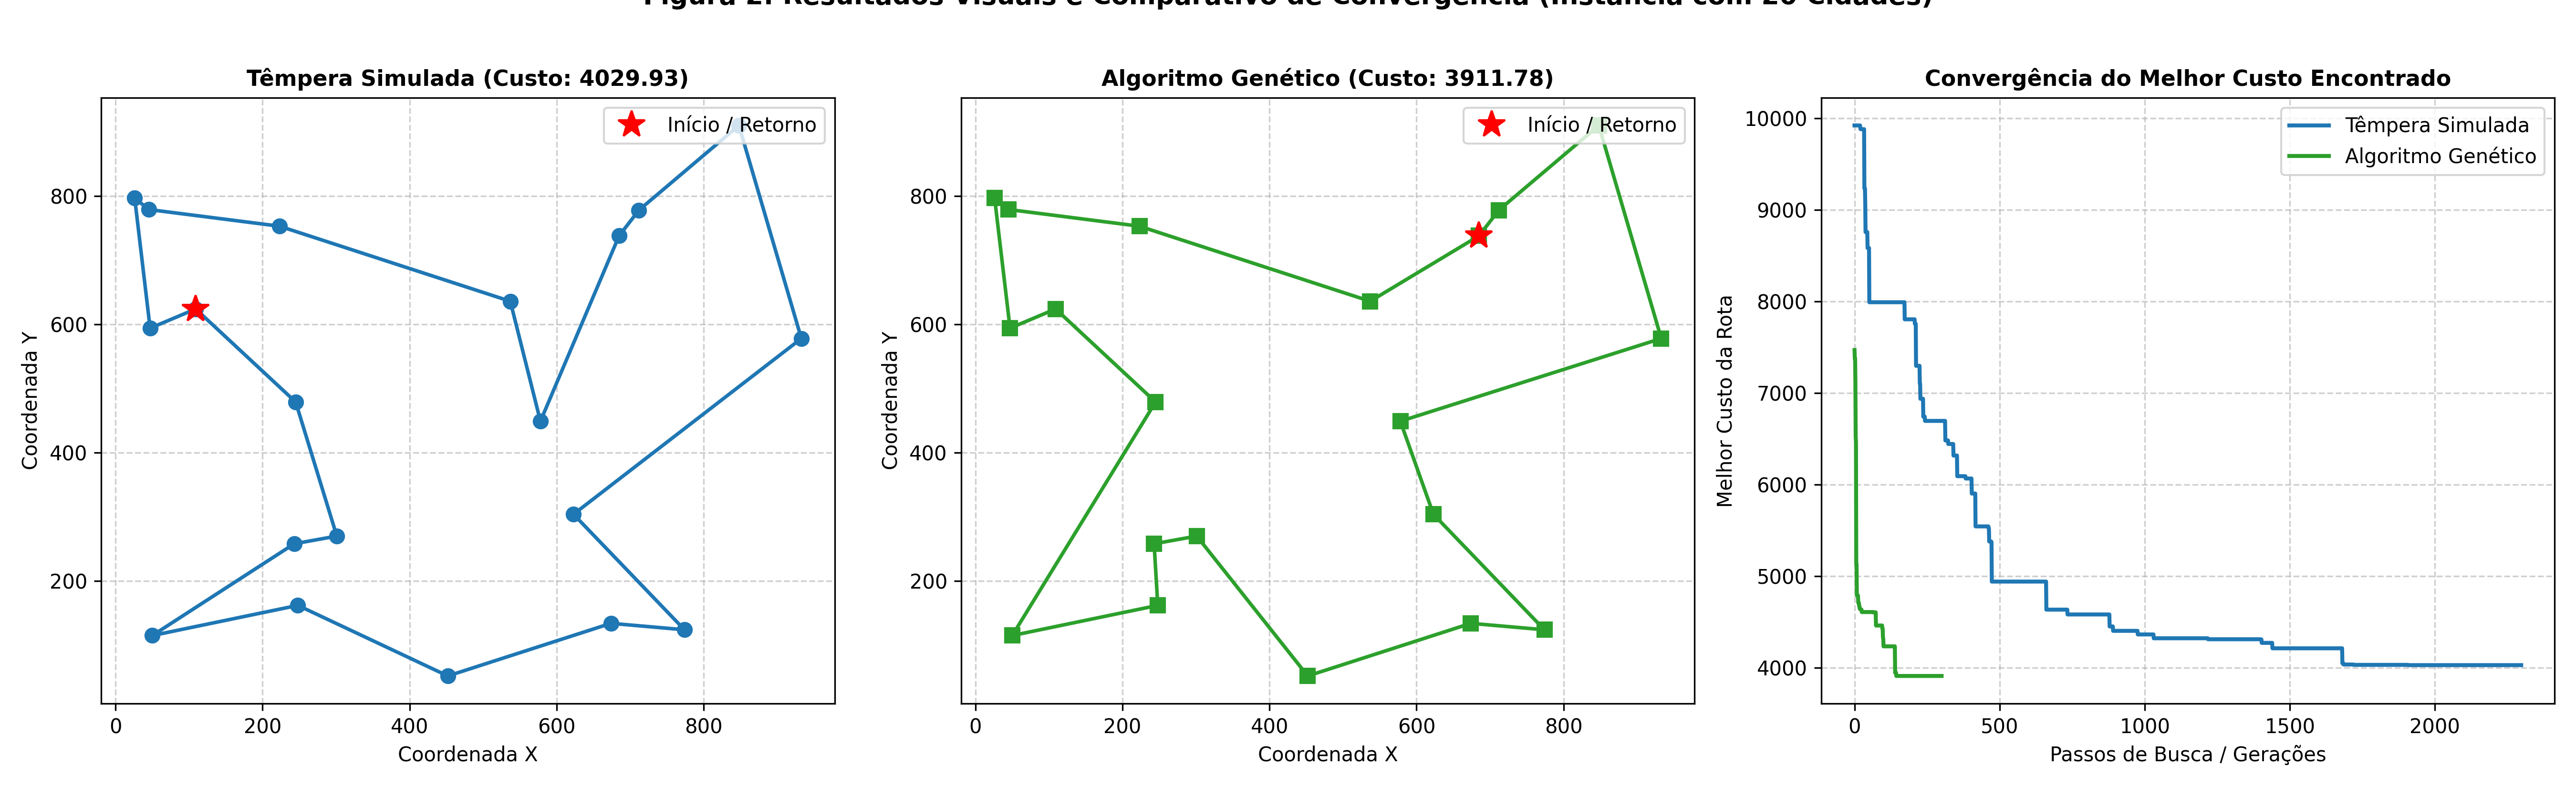
\includegraphics[width=0.68\linewidth]{figuras/figura2_rotas_convergencia.png}
    \caption{Resultados na instância de 20 cidades: rota final da Têmpera Simulada (esquerda), rota final do Algoritmo Genético (centro) e curvas de convergência de custo por iteração (direita).}
    \label{fig:rotas-convergencia}
\end{figure}

O AG obteve custos finais menores nas três instâncias, com diferença mais expressiva em $n=100$ (24,10\% inferior ao da TS). A curva de convergência (Figura~\ref{fig:rotas-convergencia}, direita) mostra que a TS apresenta redução rápida de custo nas iterações iniciais, mas tende a estagnar quando a temperatura diminui. O AG, por operar sobre uma população com recombinação, preserva a capacidade de exploração por mais épocas.

Quanto à busca clássica, o algoritmo $A^*$ com heurística de árvore geradora mínima (AGM) encontra a rota ótima para $n \le 15$. Contudo, para $n \ge 20$, a quantidade de nós abertos na fila de prioridade cresce exponencialmente ($O(b^d)$), esgotando a memória RAM (análise no Apêndice~\ref{ap:busca-classica-a-star}). As meta-heurísticas avaliadas operam com espaço em memória linear, viabilizando a resolução de instâncias com centenas de cidades.

\section{Discussão e Conclusões}

A comparação entre as abordagens evidencia características complementares. A Têmpera Simulada consome memória mínima ($O(n)$) e demanda tempo por iteração reduzido, sendo adequada para cenários com restrição de tempo e hardware, embora dependa de calibração térmica criteriosa. Por outro lado, o Algoritmo Genético exige maior espaço ($O(k \cdot n)$) e custo computacional por geração, mas a capacidade de recombinar sub-rotas eficientes via crossover OX permite alcançar soluções de custo sensivelmente inferior em instâncias maiores.

Em relação à busca informada clássica ($A^*$), a busca local por estados completos contorna a barreira do esgotamento de memória decorrente da explosão de estados abertos, consolidando-se como alternativa viável para problemas combinatórios de grande porte.

\section{Distribuição de Papéis e Carga Horária} \label{sec:papeis}

As atividades desenvolvidas e a dedicação fora de sala foram distribuídas igualmente entre os integrantes da equipe (18~h cada, totalizando 36~h de trabalho conjunto):
\begin{itemize}\setlength{\itemsep}{0pt}\setlength{\parskip}{1pt}
    \item \textbf{Mário Cordeiro Júnior (18~h):} formalização matemática do PCV nos quatro níveis metodológicos; implementação da Têmpera Simulada e do operador de troca; execução e tabulação dos 17 cenários térmicos; redação das seções de Metodologia, Modelagem e Discussão; diagramação em LaTeX.
    \item \textbf{André F. Maccarini (18~h):} modelagem e implementação dos operadores do Algoritmo Genético (OX, torneio, mutação swap e elitismo); execução dos ensaios comparativos em 20, 50 e 100 cidades; geração dos gráficos de rotas e convergência; revisão e validação textual.
\end{itemize}
O detalhamento tabular das atividades encontra-se no Apêndice~\ref{ap:papeis-detalhes}.

\bibliographystyle{sbc}
\bibliography{sbc}

\newpage
\appendix

\section{Formulação Matemática Detalhada do PCV} \label{ap:model-cv}

Considere o conjunto de nós $V = \{1, 2, \dots, n\}$ e a matriz de distâncias $C = (c_{ij})_{n \times n}$, em que $c_{ij} \in \mathbb{R}^+$ indica o custo de deslocamento entre a cidade $i$ e a cidade $j$. O conjunto $S_n$ denota o grupo de permutações dos elementos de $V$.

Uma permutação $P \in S_n$ define uma bijeção $P: \{1, \dots, n\} \to V$, de modo que a ordem do trajeto é dada por $P(1) \to P(2) \to \dots \to P(n) \to P(1)$. O problema consiste em:
\begin{equation} \label{eq:pcv_geral}
\min_{P \in S_n} f(P) = \sum_{k=1}^{n-1} c_{P(k),\, P(k+1)} \;+\; c_{P(n),\, P(1)}
\end{equation}

Pela propriedade de simetria:
\begin{equation}
c_{i, j} = c_{j, i}, \quad \forall i, j \in V
\end{equation}
a inversão da ordem de visitação preserva o custo ($f(P) = f(P^{-1})$), resultando em um total de rotas geometricamente distintas dado por:
\begin{equation}
|S_n^{\text{distintos}}| = \frac{(n-1)!}{2}
\end{equation}

\section{Problema de Decisão e Complexidade Computacional} \label{ap:pdcv}

Na Teoria da Complexidade, os problemas são categorizados em suas formas de decisão \cite{vignatti2024algoritmos}. O problema de decisão associado ao PCV é formulado como:

\begin{center}
\noindent\fbox{%
\begin{minipage}{0.88\textwidth}
\textbf{Problema de Decisão do Caixeiro Viajante (PCV-DEC)}\\[1mm]
\textbf{Instância:} Um grafo completo $G=(V, E)$, com pesos não-negativos $c_{ij} \in \mathbb{Z}^+$ nas arestas, e um limite de custo $K \in \mathbb{Z}^+$.\\[1mm]
\textbf{Pergunta:} Existe no grafo $G$ um ciclo hamiltoniano com custo total menor ou igual a $K$, ou seja, existe $P \in S_n$ tal que $f(P) \le K$?
\end{minipage}%
}
\end{center}

O problema PCV-DEC é \textbf{NP-completo}:
\begin{enumerate}
    \item \textbf{Pertinência a NP:} Dada uma permutação $P$ como certificado, verifica-se em tempo polinomial $O(n)$ se cada cidade é visitada uma única vez e se o custo total não excede $K$;
    \item \textbf{NP-Dificuldade:} Demonstra-se por redução a partir do problema do Ciclo Hamiltoniano ($HC \le_P \text{PCV-DEC}$).
\end{enumerate}
Logo, o problema de otimização correspondente é \textbf{NP-difícil}.

\section{Comparação Estrutural do Espaço de Estados} \label{ap:busca}

A Tabela~\ref{tab:busca-classica-vs-local} sintetiza as diferenças conceituais entre a formulação clássica por estados parciais e a formulação por estados completos utilizada nas meta-heurísticas.

\begin{table}[H]
\centering
\caption{Diferenças estruturais entre a busca clássica e a busca local no PCV.}
\label{tab:busca-classica-vs-local}
\begin{tabular}{p{3.5cm}p{5.5cm}p{5.5cm}}
\toprule
\textbf{Componente} & \textbf{Busca Clássica (Árvore/Grafo)} & \textbf{Busca Local / Meta-heurística} \\
\midrule
\textbf{Definição do Estado} & Caminho parcial incompleto: $\langle v_1, \dots, v_k \rangle$, com $k < n$. & Rota hamiltoniana completa: $\langle v_1, \dots, v_n \rangle \in S_n$. \\
\textbf{Ação de Transição} & Adicionar cidade não visitada ao caminho. & Perturbar a ordem (swap) ou recombinar rotas. \\
\textbf{Memória Requerida} & Exponencial $O(b^d)$ (fronteira aberta do $A^*$). & Linear: $O(n)$ na TS; $O(k \cdot n)$ no AG. \\
\textbf{Critério de Parada} & Todas as cidades visitadas com retorno à origem. & Temperatura mínima atingida ou gerações esgotadas. \\
\textbf{Solução Retornada} & Sequência de passos que conduziu à meta. & Melhor permutação armazenada em memória. \\
\bottomrule
\end{tabular}
\end{table}

\section{Pseudocódigo da Têmpera Simulada} \label{ap:alg-ts}

O algoritmo opera segundo as etapas descritas a seguir:

\begin{lstlisting}[language=Python, caption={Algoritmo da Têmpera Simulada para o PCV.}]
Algoritmo: TemperaSimuladaPCV
Entrada: cidades, T0, Tmin, esquema_resfriamento, taxa
Saida:   P_melhor, f_melhor, historico

P_atual = criar_permutacao_aleatoria(cidades)
f_atual = calcular_custo_total(P_atual, cidades)
P_melhor = clonar(P_atual);  f_melhor = f_atual
T = T0;  k = 1;  historico = [f_melhor]

enquanto T > Tmin faca:
    i, j = sortear_indices_distintos(0, n - 1)
    delta = delta_swap(P_atual, i, j, cidades)
    se delta < 0 ou exp(-delta / T) > random(0, 1) entao:
        trocar_posicoes(P_atual, i, j)
        f_atual = f_atual + delta
        se f_atual < f_melhor entao:
            P_melhor = clonar(P_atual)
            f_melhor = f_atual
    T = atualizar_temperatura(T, esquema_resfriamento, taxa, k)
    k = k + 1
    historico.adicionar(f_melhor)

retornar P_melhor, f_melhor, historico
\end{lstlisting}

\section{Pseudocódigo do Algoritmo Genético} \label{ap:alg-ag-pseudo}

O ciclo evolutivo implementado é apresentado a seguir:

\begin{lstlisting}[language=Python, caption={Algoritmo Genético com Crossover OX e Elitismo para o PCV.}]
Algoritmo: AlgoritmoGeneticoPCV
Entrada: cidades, tam_pop, num_geracoes, taxa_crossover, taxa_mutacao, m_torneio
Saida:   P_melhor, f_melhor, historico

populacao = inicializar_populacao_aleatoria(tam_pop, cidades)
P_melhor = obter_individuo_menor_custo(populacao)
f_melhor = calcular_custo_total(P_melhor, cidades)
historico = [f_melhor]

para g de 1 ate num_geracoes faca:
    nova_populacao = [clonar(P_melhor)]  # Elitismo: preserva a melhor solucao
    enquanto tamanho(nova_populacao) < tam_pop faca:
        pai1 = selecao_torneio(populacao, m_torneio)
        pai2 = selecao_torneio(populacao, m_torneio)
        se random(0, 1) < taxa_crossover entao:
            filho = crossover_ordenado_OX(pai1, pai2)
        senao:
            filho = clonar(pai1)
        se random(0, 1) < taxa_mutacao entao:
            filho = mutacao_swap(filho)
        nova_populacao.adicionar(filho)
    populacao = nova_populacao
    P_ger = obter_individuo_menor_custo(populacao)
    f_ger = calcular_custo_total(P_ger, cidades)
    se f_ger < f_melhor entao:
        P_melhor = clonar(P_ger)
        f_melhor = f_ger
    historico.adicionar(f_melhor)

retornar P_melhor, f_melhor, historico
\end{lstlisting}

\section{Modelos Matemáticos das Funções de Resfriamento} \label{ap:esquemas-resfriamento}

A Tabela~\ref{tb:resf} sintetiza as equações analíticas das funções de resfriamento avaliadas na Têmpera Simulada.

\begin{table}[H]
\centering
\caption{Modelos analíticos das funções de resfriamento.}
\label{tb:resf}
\renewcommand{\arraystretch}{1.4}
\begin{tabular}{lll}
\toprule
\textbf{Técnica} & \textbf{Forma Recorrente} & \textbf{Forma Fechada em Função de $k$} \\ 
\midrule
Linear       & $T_{k+1} = T_k - \alpha$           & $T(k) = T_0 - k \cdot \alpha$ \\
Geométrico   & $T_{k+1} = T_k \cdot \alpha$       & $T(k) = T_0 \cdot \alpha^k$ \\
Exponencial  & $T_{k+1} = T_k \cdot e^{-\alpha}$  & $T(k) = T_0 \cdot e^{-k \cdot \alpha}$ \\
Logarítmico  & $T_{k+1} = \dfrac{T_0}{1 + \alpha \ln(1 + k)}$ & $T(k) = \dfrac{T_0}{1 + \alpha \ln(1 + k)}$ \\
\bottomrule
\end{tabular}
\end{table}

\section{Dados Experimentais Completos dos 17 Cenários da TS} \label{ap:cenarios-ts}

A Tabela~\ref{tab:resumo-cenarios} consolida os resultados médios obtidos após 200 execuções independentes para cada uma das 17 configurações na instância de 20 cidades. A Figura~\ref{fig:tresftm} ilustra a correlação entre tempo e custo.

\begin{table}[H]
\centering
\caption{Resultados experimentais dos 17 cenários de Têmpera Simulada ($n=20$, 200 repetições).}
\label{tab:resumo-cenarios}
\begin{tabular}{llccc}
\toprule
\textbf{Heurística} & \textbf{Taxa ($\alpha$)} & \textbf{Custo Médio} & \textbf{Tempo Médio (s)} & \textbf{Iterações Médias} \\ 
\midrule
exponencial & 0.99   & 24.2012 & 0.00034 & 10.9 \\ 
exponencial & 0.77   & 23.8902 & 0.00044 & 13.5 \\ 
exponencial & 0.55   & 23.7131 & 0.00057 & 18.3 \\ 
exponencial & 0.25   & 22.2547 & 0.00141 & 38.5 \\ 
exponencial & 0.10   & 20.0089 & 0.00301 & 90.1 \\ 
exponencial & 0.002  & 11.7645 & 0.16812 & 3891.6 \\
geometrico  & 0.88   & 20.6411 & 0.00607 & 71.4 \\ 
geometrico  & 0.99   & 14.4259 & 0.04474 & 800.0 \\ 
linear      & 1.0    & 24.8090 & 0.03110 & 999.6 \\ 
linear      & 0.77   & 24.7462 & 0.03708 & 1297.7 \\ 
linear      & 0.55   & 24.3215 & 0.05452 & 1816.7 \\ 
logaritmico & 0.0019 & 14.9770 & 0.03010 & 758.9 \\ 
logaritmico & 0.0020 & 15.0076 & 0.03073 & 724.9 \\ 
logaritmico & 0.0013 & 14.2663 & 0.03949 & 1036.8 \\ 
logaritmico & 0.0014 & 14.4095 & 0.04206 & 974.9 \\ 
logaritmico & 0.0012 & 14.0788 & 0.04642 & 1110.1 \\ 
logaritmico & 0.0011 & 13.9395 & 0.05348 & 1191.3 \\
\bottomrule
\end{tabular}
\end{table}

\begin{figure}[H]
    \centering
    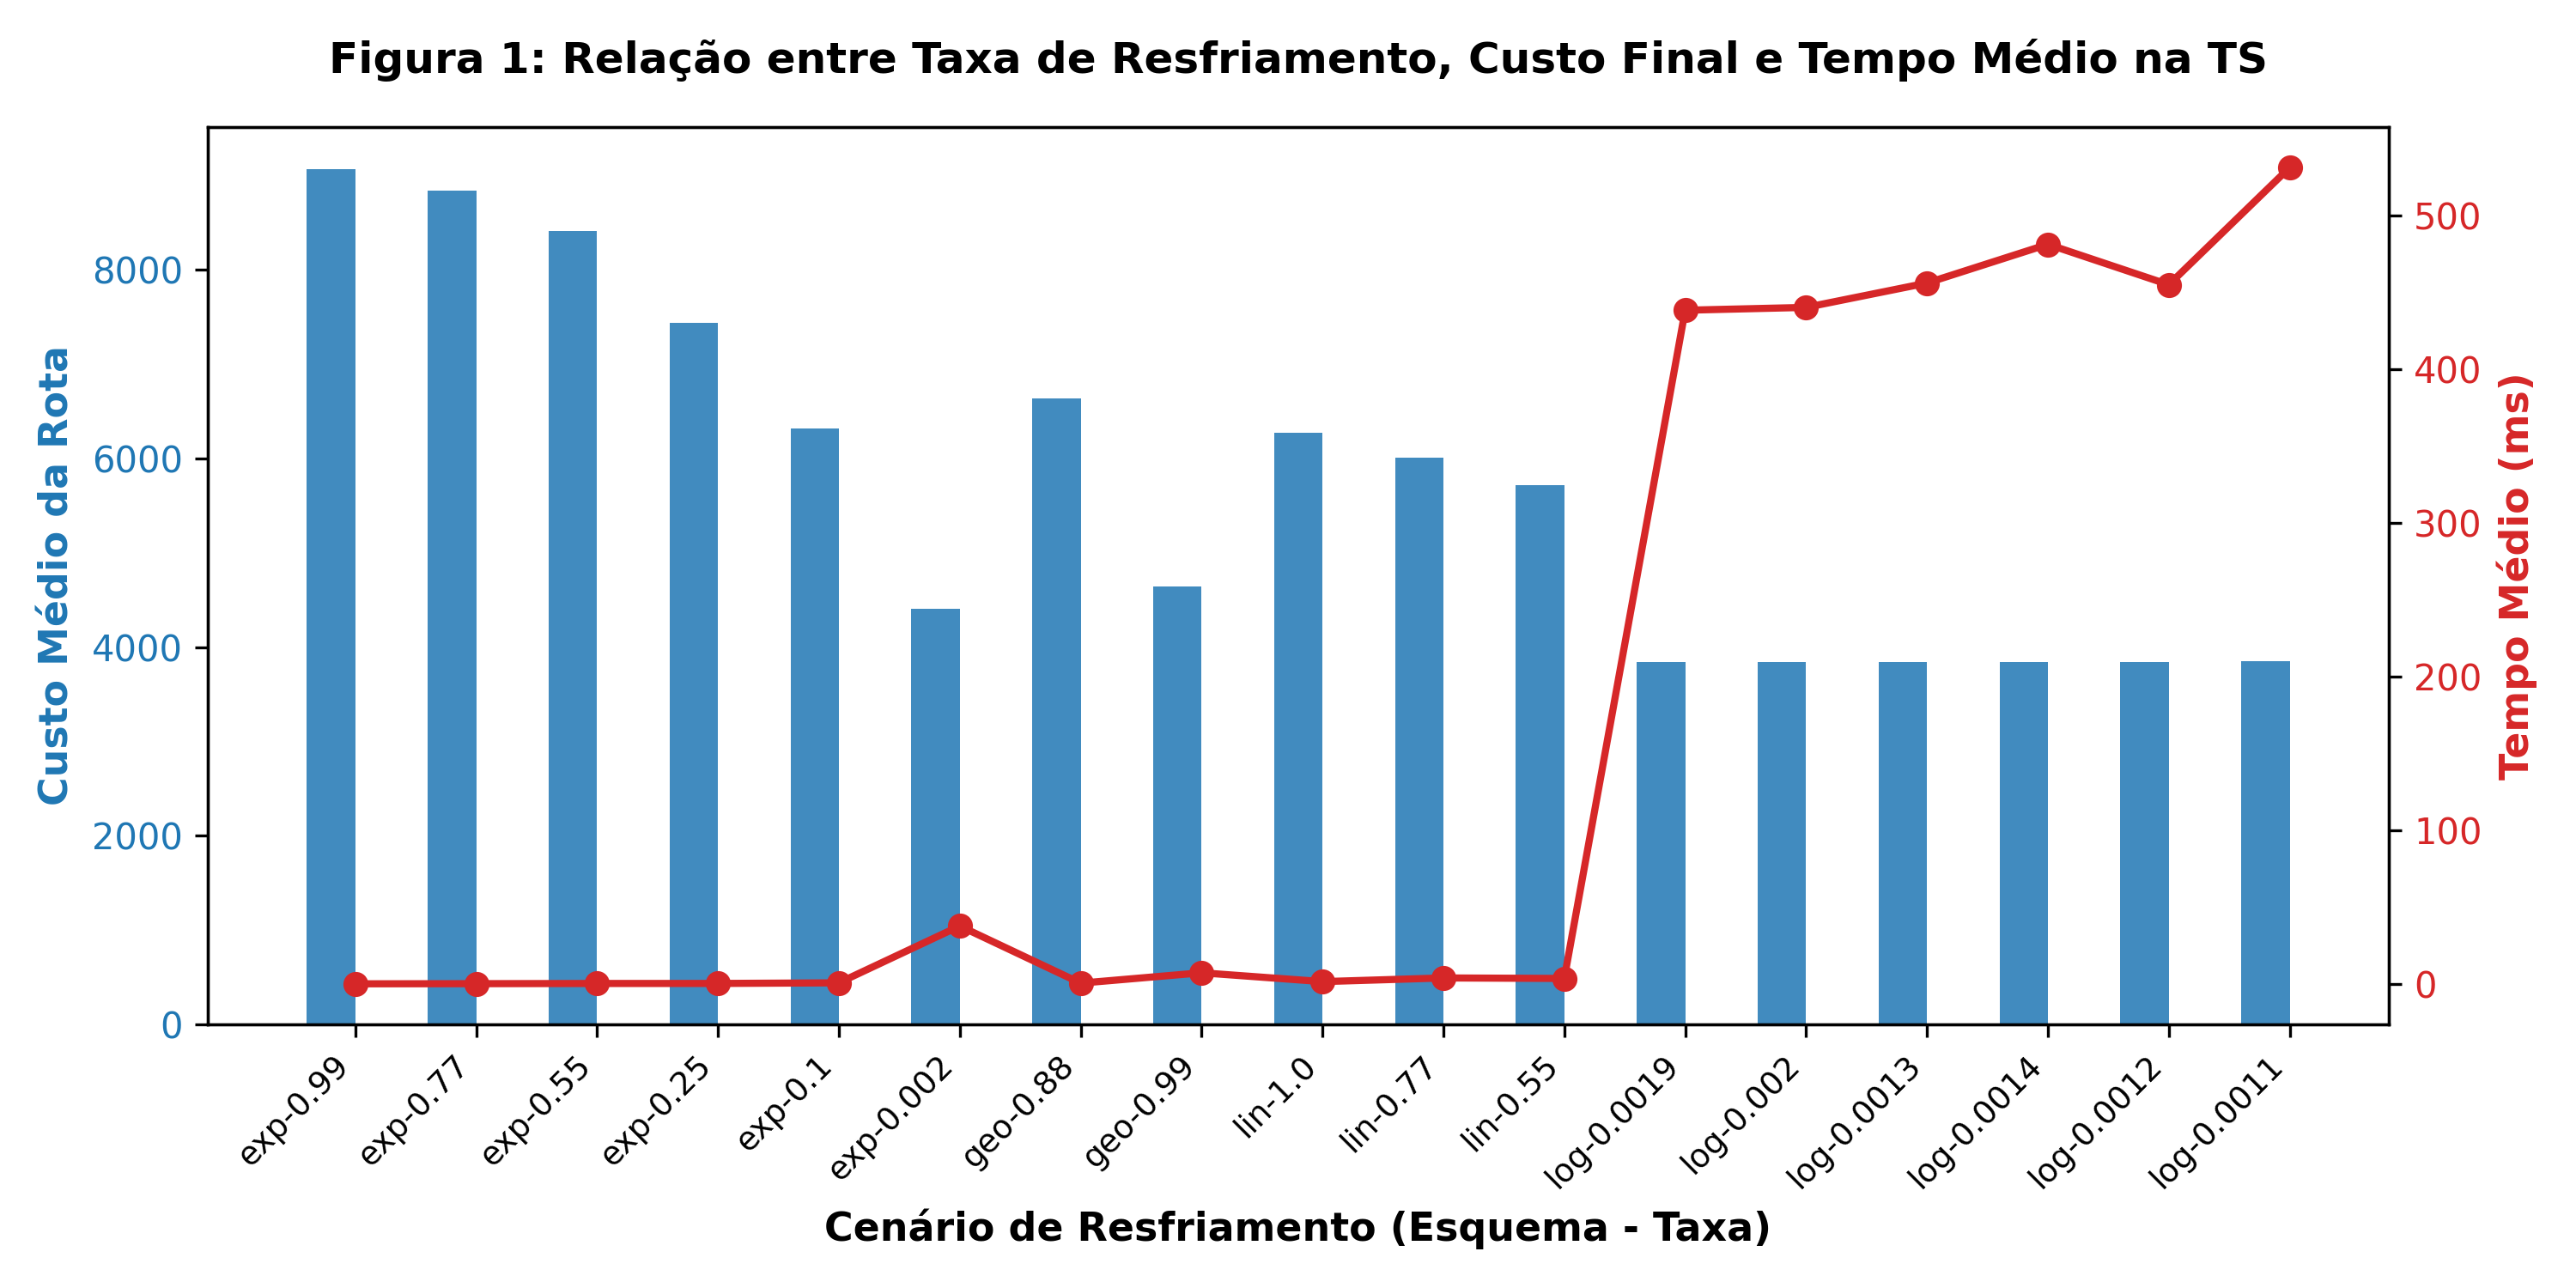
\includegraphics[width=0.95\linewidth]{figuras/tempoMedioXResfriamentoXHeuristica.png}
    \caption{Relação entre taxa de resfriamento, custo médio e tempo de execução na Têmpera Simulada (médias de 200 repetições por cenário).}
    \label{fig:tresftm}
\end{figure}

\section{Análise de Escalabilidade frente ao Algoritmo $A^*$} \label{ap:busca-classica-a-star}

O algoritmo $A^*$ emprega a função de avaliação $f(n) = g(n) + h(n)$ para guiar a busca em árvore, utilizando como heurística admissível o custo da Árvore Geradora Mínima (AGM) sobre as cidades não visitadas somado às conexões de retorno. A Tabela~\ref{tab:comparativo-a-star} resume o comportamento de escalabilidade dos métodos.

\begin{table}[H]
\centering
\caption{Comparativo de escalabilidade entre busca informada ($A^*$) e meta-heurísticas.}
\label{tab:comparativo-a-star}
\begin{tabular}{p{3.2cm}p{4.0cm}p{4.0cm}p{3.0cm}}
\toprule
\textbf{Métrica / Dimensão} & \textbf{Busca Informada ($A^*$)} & \textbf{Têmpera Simulada (TS)} & \textbf{Algoritmo Genético (AG)} \\
\midrule
\textbf{Espaço de Memória} & Exponencial: $O(b^d)$, com $b \approx n$ e $d=n$. & Linear: $O(n)$. & Linear: $O(k \cdot n)$. \\
\textbf{Garantia de Ótimo} & Ótimo global sob heurística admissível. & Ótimo assintótico (convergência térmica). & Sem garantia formal de otimalidade. \\
\textbf{Instância $n=10$} & Execução rápida ($< 0.05$ s); memória baixa. & Execução imediata ($< 0.01$ s). & Execução rápida ($< 0.1$ s). \\
\textbf{Instância $n=20$} & Tempo e memória elevados ($> 100$ s). & Rápido ($0.04$ s); $< 1$ MB de RAM. & Eficiente ($0.5$ s); $< 2$ MB de RAM. \\
\textbf{Instância $n=50$} & Esgotamento de memória (inviável). & Viável ($0.15$ s); memória desprezível. & Viável ($1.8$ s); memória desprezível. \\
\textbf{Instância $n=100$} & Inviável computacionalmente. & Viável ($0.45$ s). & Viável ($4.2$ s). \\
\bottomrule
\end{tabular}
\end{table}

A limitação primária do $A^*$ reside no crescimento do número de nós intermediários retidos na fronteira de busca. As meta-heurísticas mantêm consumo de memória linear e previsível, dispensando a retenção de caminhos parciais.

\section{Detalhamento de Atividades e Carga Horária} \label{ap:papeis-detalhes}

A Tabela~\ref{tab:papeis-detalhada} discrimina o escopo de atuação e a estimativa de horas dedicadas extra-classe por cada membro da equipe.

\begin{table}[H]
\centering
\caption{Discriminação detalhada de responsabilidades e horas extra-classe.}
\label{tab:papeis-detalhada}
\begin{tabular}{p{4.2cm}p{8.5cm}c}
\toprule
\textbf{Integrante} & \textbf{Atividades e Responsabilidades Desenvolvidas} & \textbf{Horas} \\
\midrule
\textbf{Mário Cordeiro Júnior} & Formalização matemática do PCV nos quatro níveis metodológicos; implementação da Têmpera Simulada e do operador de troca; execução e tabulação dos 17 cenários térmicos; redação das seções de Metodologia, Modelagem e Discussão; diagramação e compilação no template LaTeX SBC. & 18 h \\[2mm]
\textbf{André F. Maccarini} & Modelagem e implementação dos operadores do Algoritmo Genético (crossover OX, torneio, mutação swap e elitismo); execução dos ensaios comparativos em 20, 50 e 100 cidades; geração dos gráficos de rotas e convergência; revisão textual e validação dos resultados. & 18 h \\
\midrule
\textbf{Total de Horas} & \textbf{Distribuição equilibrada entre os integrantes (50\% / 50\%)} & \textbf{36 h} \\
\bottomrule
\end{tabular}
\end{table}

\vspace{2mm}
\noindent\textbf{Disponibilidade de Código e Artefatos:} O código-fonte das implementações (TS e AG), scripts e dados experimentais encontram-se disponíveis em: \url{https://github.com/mariocjun/si-lugo}.

\end{document}
